
\documentclass[11pt]{article}

%Menge: \mathbb{R}

\usepackage[ngerman]{babel}
\usepackage{amsmath} %align, für = untereinander einfach &=
\usepackage{amssymb}
\usepackage{amsthm}
\usepackage{listings}
\usepackage[utf8]{inputenc}
\usepackage{graphicx}
\usepackage{esvect}
\graphicspath{ {./images/} }
\usepackage{tikz}         % For arrow and dots in \xvec
\usepackage[left=2.30cm, right=2.30cm, top=1.70cm, bottom=2.00cm]{geometry}

% --- Macro \xvec
\makeatletter
\newlength\xvec@height%
\newlength\xvec@depth%
\newlength\xvec@width%
\newcommand{\xvec}[2][]{%
	\ifmmode%
	\settoheight{\xvec@height}{$#2$}%
	\settodepth{\xvec@depth}{$#2$}%
	\settowidth{\xvec@width}{$#2$}%
	\else%
	\settoheight{\xvec@height}{#2}%
	\settodepth{\xvec@depth}{#2}%
	\settowidth{\xvec@width}{#2}%
	\fi%
	\def\xvec@arg{#1}%
	\def\xvec@dd{:}%
	\def\xvec@d{.}%
	\raisebox{.2ex}{\raisebox{\xvec@height}{\rlap{%
				\kern.05em%  (Because left edge of drawing is at .05em)
				\begin{tikzpicture}[scale=1]
				\pgfsetroundcap
				\draw (.05em,0)--(\xvec@width-.05em,0);
				\draw (\xvec@width-.05em,0)--(\xvec@width-.15em, .075em);
				\draw (\xvec@width-.05em,0)--(\xvec@width-.15em,-.075em);
				\ifx\xvec@arg\xvec@d%
				\fill(\xvec@width*.45,.5ex) circle (.5pt);%
				\else\ifx\xvec@arg\xvec@dd%
				\fill(\xvec@width*.30,.5ex) circle (.5pt);%
				\fill(\xvec@width*.65,.5ex) circle (.5pt);%
				\fi\fi%
				\end{tikzpicture}%
	}}}%
	#2%
}
\makeatother

\usepackage{blindtext}
%\usepackage{bookman}

% --- Override \vec with an invocation of \xvec.
\let\stdvec\vec
\renewcommand{\vec}[1]{\xvec[]{#1}}
% --- Define \dvec and \ddvec for dotted and double-dotted vectors.
\newcommand{\dvec}[1]{\xvec[.]{#1}}
\newcommand{\ddvec}[1]{\xvec[:]{#1}}

%eigene Befehle:
\newcommand{\R}{\mathbb{R}}
\newcommand{\nablavec}{\vec{\nabla}}

\title{Theoretische Physik 1}

\date{\today}
\begin{document}
\lstset{language=Java}
\author{Tom Herrmann}
\linespread{1.55}
\maketitle
\tableofcontents
\newpage

\section{Einleitung}
	Gliederung:
	\begin{itemize}
		\item \textbf{Mathematische Grundlagen:}\\Vektoren, krummlinige Koordinatensysteme, Differential- und Integralrechnung, partielle Ableitungen, Vektoranalysis, Gradient, Diverenz, Rotation, lineare gewöhnliche Differentialgleichungen, Matrizen und Tensoren, Fourier-Transformation, komplexe Zahlen, Wahrscheinlichkeit.
		\item \textbf{Grundlagen der Mechanik:} Kinematik und Dynamik von Massenpunktsystemen, Newtonsche Axiome, Arbeit, konservative Kräfte, Schwingungen, Zentralfeld, Kepler-Problem, beschleunigte Bezugssysteme
		\item \textbf{Spezielle Relativitätstheorie:}  Lorentz-Transformation und kinematische Konsequenzen, Minkowski-Raum, Vierer-Impuls, relativistische Bewegungsgleichung, Energie-Impuls-Vektor, Äquivalenz von Masse und Energie
		\item \textbf{Wärmelehre: } Boltzmann Verteilung, Entropie, Irreversibilität
	\end{itemize}
		\textbf{Wenn man eine Fettgedruckte Größe in den Übungsaufgaben sieht ist damit ein Vektor gemeint}
\part{Vorlesung 1}
	$\#$ = Anzahl
	\section{Grundlagen}
	\subsection{Vektorrechnung}
		Vektoren sind gerichtete Größen deren Komponenten bei Drehung oder allgemeiner Koordinaten Transformationen gewisse transformationseigenschaften besitzen. \\
		Skalare sind dabei invariant unter Koordinatentransformation. (z.B: Masse, Ladung, Temperatur)\\
		Ortsvektor $\vec{r}$, Geschwindigkeit $\vec{v} = \frac{d\vec{r}}{dt} = \frac{d^2\vec{r}}{dt^2} $\\
		Vektoren haben eine Richtung und eine Länge.
	\subsection{Formale Schreibweise Ableitungen}
		Ableitung können sowas als $f`$ geschrieben werden als auch als $\dot{f}$ somit kann die Geschwindigkeit $\vec{v}$ als die Ableitung der Position ausgedrückt werden $\vec{v}$ = $\vec{\dot{x}}$.
	\subsection{Drehung}
	$\vec{a} = (a_x, a_y) = (x, y)$\\
	$\vec{a} = (a_u, a_v) = (u, v)$ dabei ist für u und v das Koordinatensystem einfach nur um einen bestimmten Winken $\varphi$ gedreht.\\
	\[u = x cos \varphi + y sin \varphi\]
	\[v = - x sin \varphi + y cos \varphi\]
	Länge von: \[\vec{a} = \sqrt{u^2+ v^2} = [\left(x cos \varphi + y sin \varphi)^2 (- x sin \varphi + y cos \varphi)^2\right]^\frac{1}{2}\]
	\[	[x^2 cos^2 \varphi + y^2 sin^2\varphi+xy cis \varphi sin \varphi + x^2 sin^2 \varphi + y^2 cos^2 \varphi - 2xy sin \varphi cos \varphi]^\frac{1}{2}\]
	\[ [x^2(cos^2\varphi + sin^2 \varphi) + y^2 sin^2\varphi + cos^2 \varphi]^\frac{1}{2} \]
	\[ \sqrt{x^2 + y^2} \] \qed \\
\subsubsection{Drehung als Matrix Multiplikation:} 
$\left( \begin{array}{c}
	u \\ 
	v
\end{array} \right)
= \left( \begin{array}{cc}
	cos \varphi & sin \varphi \\ 
	-sin \varphi & cos \varphi
\end{array} \right)
  \left( \begin{array}{ccc}
 	x \\ 
 	y
 \end{array} \right)
= \frac{2}{2} = A_{ij} x_j $  

\part{Vorlesung 2}
	\subsection{Basis der Vektorrechnung}
	Mathematisch abstrakt ist ein linearer oder Vektorraum ein "Körper" von Elementen $\vec{a}, \vec{b}, \vec{c}$, im dem eine Addition und eine ultiplikation mit skalaren $\alpha$ definiert ist.
		
		\subsubsection{Basis ausrechnung}
			\begin{itemize}
				\item Die Anzahl der Vektoren stimmt überein mit der Dimension des Vektorraumes.
				\item Die Vektoren sind linear unabhängig.
			\end{itemize}
		\subsubsection{Addition}
		\[	\left(\begin{array}{c}
				1\\ 
				2
			\end{array} \right) + \left(\begin{array}{c}
			3\\ 
			5
		\end{array} \right) =	\left(\begin{array}{c}
		1 + 3\\ 
		2 + 5
	\end{array} \right) = \left(\begin{array}{c}
	4\\ 
	7
\end{array} \right) \]
		\subsubsection{Subtraktion}
		\[	\left(\begin{array}{c}
				3\\ 
				4
			\end{array} \right) - \left(\begin{array}{c}
			2\\ 
			5
		\end{array} \right) =
	\left(\begin{array}{c}
		3 - 2\\ 
		4 - 5
	\end{array} \right) = \left(\begin{array}{c}
	1\\ 
	-1
\end{array} \right) \]
		\subsubsection{Multiplikation}
		\[	a * \vec{v} = 5 * \left(\begin{array}{c}
				2\\ 
				1\\
				3
			\end{array} \right) = \left(\begin{array}{c}
			5 * 2 \\ 
			5 * 1 \\
			5 * 3
			\end{array} \right) =
			\left(\begin{array}{c}
			10\\ 
			5\\
			15
			\end{array} \right) 	\]  
			Bei der Division läuft das ganze dann fast genau so ab einfach nur 5 in den als zähler der jeweiligen Koordinate schreiben.
		\subsubsection{Skalarprodukt}
			\[ \vec{a} \circ \vec{b} = |\vec{a}| \circ |\vec{b}| = \begin{pmatrix} a_1 \\ a_2 \\ a_3 \end{pmatrix} \circ \begin{pmatrix} b_1 \\ b_2 \\ b_3 \end{pmatrix} = a_1 \cdot b_1 + a_2 \cdot b_2 + a_3 \cdot b_3 \]
		\subsection{Eigenschaften von Rechenoperationen}
		Kommutativität $\vec{a} + \vec{b} = \vec{b} + \vec{a}$\\
		Distributivität $\lambda * (\vec{a} + \vec{b}) = (\vec{a} + \vec{b}) * \lambda$\\
		Homogenität (gemischtes Assoziativgesetz) $\alpha(\vec{a} + \vec{b} = (\alpha \vec{a}) * \vec{b} =  \vec{a} * (\alpha \vec{b})$
		
		
		\subsubsection{Schwarzsche Ungleichung}
			$|\vec{a} * \vec{b}| \leq |\vec{a}| |\vec{b}|$
			
		\subsubsection{Projektion auf die Richtung \vec{b}}
			$a_b := a cos(\varphi) = \vec{a} * \vec{b} \text{ wo } \vec{b} := \frac{\vec{b}}{|\vec{b}|}$ der Einheutsvektor in $\vec{b}$ Richtung ist. (Also soll hier b der Einheitsvektor sein)\\
			Abstrake Definition eines Skalarproduktes mit obigen Eigenschaften und zusätzlichen $\vec{a}*\vec{a} > 0   \exists \vec{a} \neq 0 $ (positiv definiert)\\
		\part{Vorlesung 3}
			\subsubsection{Vektorprodukt}
				$\vec{c} = \vec{a} \times \vec{b}$ \qquad $|\vec{c}| = c = ab$  \;  $ |sin \varphi|$
		\begin{center}
			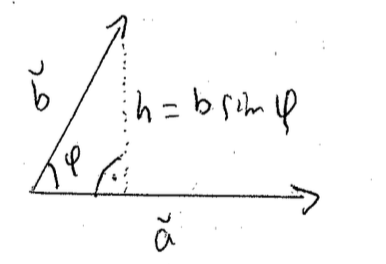
\includegraphics[scale=0.3]{vektorprodukt.png}
		\end{center}
	$\Leftarrow$ c = Fläche des von $\vec{a}$ und $\vec{b}$ aufgespannten Paralellogramms Richtung bestimmt durch \textbf{Rechtsschrauben regel}: Drehe $\vec{a}$ in Richtung $\vec{b}$
		\begin{center}
		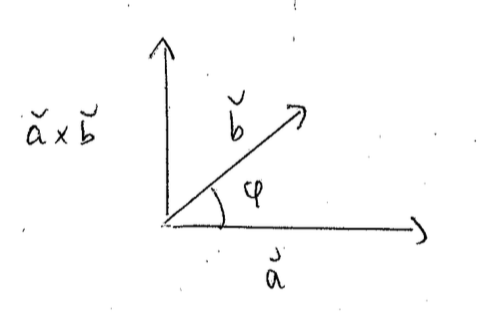
\includegraphics[scale=0.3]{vektorprodukt2.png}
	\end{center}
	\textbf{Eigenschaften:}\\
	Antikommutativität: Das heißt, bei Vertauschung der Vektoren wechselt es das Vorzeichen\\ $\vec{a}\times\vec{b} = -\, \vec{b}\times\vec{a}$\\	
	Distributivität	$\vec{a} \times (\vec{b} + \vec{c} = \vec{a} \times \vec{b} + \vec{a} \times \vec{c})$\\
	Homogenität (gemischtes Assoziativgesetz) $\alpha(\vec{a} + \vec{b} = (\alpha \vec{a}) * \vec{b} =  \vec{a} * (\alpha \vec{b})$\\
	\textbf{Sonderfälle:}\\
	$ b(\vec{a}\times\vec{b}) \times (\vec{b}\times\vec{c})  = \vec{b} \cdot \det(\vec{a},\vec{b},\vec{c}) $\\
	$ (\vec{a}\times\vec{b}) \times (\vec{a}\times\vec{c})  = \vec{a} \cdot \det(\vec{a},\vec{b},\vec{c}) $\\
	$ (\vec{a}\times\vec{b}) \times (\vec{a}\times\vec{b})  = \vec{0}$
	\subsubsection{Komonentendarstellung}
		Definiere 3 \"orthogonale\" das heißt orthogonale Einheitsvektoren\\
			$\vec{\hat{a}} , \vec{\hat{y}}, \vec{\hat{z}}$ \\der 
			im 3-Dimensionalen euklidischen Raum, mit (Schreibregel: Der einfachheit wegen lasse ich in den 2 Zeilen das Zeichen für Einheitsvektor weg, es sollte eigentlich dabei stehen) \\
			$\vec{x} * \vec{x} = \vec{y} * \vec{y} = \vec{z} * \vec{z} = 1   ; \vec{x} * \vec{y} = \vec{x} * \vec{z} = \vec{y} * \vec{z}  = 0$\\
			und\\
			$\vec{x} \times \vec{y} = \vec{z} , \vec{y} \times \vec{z} = \vec{x}, \vec{z} \times \vec{x} = \vec{y}$\\
			\textit{(Ab diesem Zeitpunkt ist die Schreibregel wieder aufgehoben)} andere häufige Schreibweisen:\\
				$\vec{e}_x, \vec{a}_y, \vec{a}_z ; \vec{e}_1, \vec{e}_2, \vec{e}_3$
				\begin{center}
					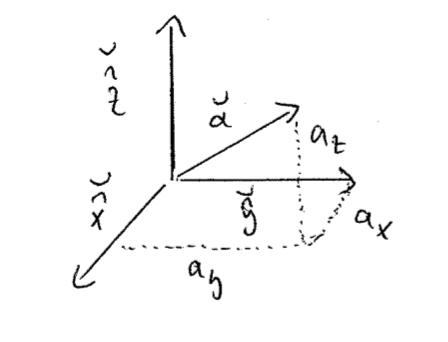
\includegraphics[scale=0.45]{komponentendarstellung.png}
				\end{center}
			$\vec{a} = a_x \vec{\hat{x}} + a_y \vec{\hat{y}} + a_z \vec{\hat{z}} = (a_x, a_y, a_z)$ mit $a_x = \vec{a} * \vec{\hat{x}}, a_y = \vec{a} * \vec{\hat{y}}, a_z = \vec{a} * \vec{\hat{z}}$
				\begin{center}
					I	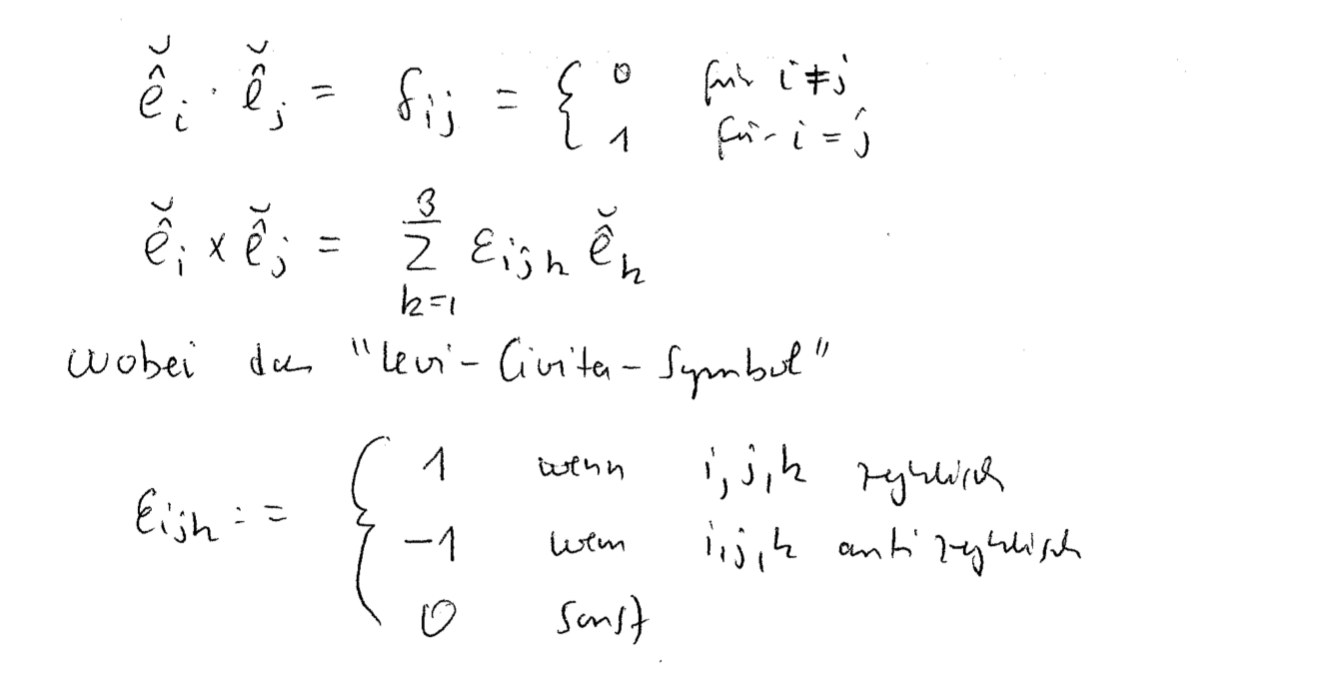
\includegraphics[scale=0.4]{Komponentendarstellung2.png}
				\end{center}
\subsubsection{Spatprodukt}
\begin{center}
	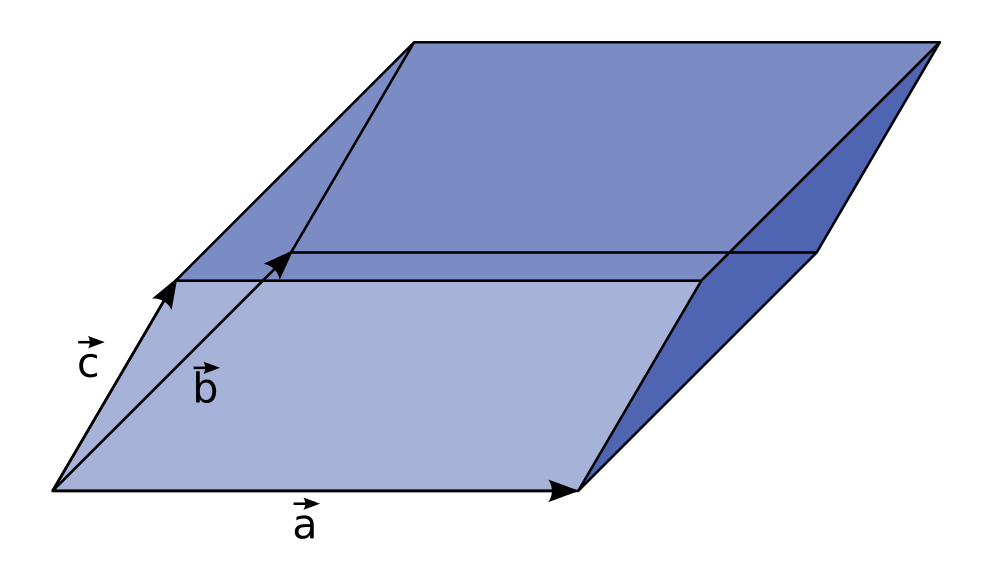
\includegraphics[scale=0.3]{1000px-Parallelepiped2.png}
\end{center}
Das Spatprodukt (\vec a, \vec b, \vec c) dreier Vektoren $\vec{a}, \vec{b}$ und $\vec{c}$ des dreidimensionalen euklidischen Vektorraums \R$^3$ kann wie folgt definiert werden: \\
	$(\vec{a},\vec{b},\vec{c}) = (\vec{a} \times \vec{b}) \cdot \vec{c}$
		\subsubsection{Eigenschaften des Spatprodukts}
			\begin{itemize}
				\item Das Spatprodukt ist \textbf{nicht kommutativ}. Der Wert ändert sich jedoch nicht, wenn man die Faktoren zyklisch vertauscht:\\
				$(\vec{a} \times \vec{b}) \cdot \vec{c} = (\vec{b} \times \vec{c}) \cdot \vec{a} = (\vec{c} \times \vec{a}) \cdot \vec{b}$
				\item Man kann das \textbf{Spatprodukt} \textbf{mit Hilfe der Determinante berechnen}. Für\\ $\vec a = \begin{pmatrix} a_1 \\ a_2 \\ a_3 \end{pmatrix},\ \vec b = \begin{pmatrix} b_1 \\ b_2 \\ b_3 \end{pmatrix},\ \vec c = \begin{pmatrix} c_1 \\ c_2 \\ c_3 \end{pmatrix}$ gilt:\\ $(\vec{a},\vec{b},\vec{c}) = \det\begin{pmatrix} a_1 & b_1 & c_1 \\ a_2 & b_2 & c_ 2 \\ a_3 & b_3 & c_3\end{pmatrix} =
				\det\begin{pmatrix} a_1 & a_2 & a_3 \\ b_1 & b_2 & b_ 3 \\ c_1 & c_2 & c_3 \end{pmatrix}$
				\item Die \textbf{Multiplikation} mit einem Skalar $\alpha \in \mathbb{R}$ ist \textbf{assoziativ }\\
					$( \alpha \cdot \vec{a}, \vec{b}, \vec{c} ) = \alpha \cdot ( \vec{a}, \vec{b}, \vec{c} )$
				\item Es gilt ein \textbf{Distributivgesetz:}\\
				$( \vec{a}, \vec{b}, \vec{c} + \vec{d} ) = ( \vec{a}, \vec{b}, \vec{c} ) + ( \vec{a}, \vec{b}, \vec{d} )$
				\item Invarianz unter zyklischer Vertauschung: \\
				$(\vec{a} \times \vec{b}) * \vec{c} = (\vec{b} \times \vec{c}) * \vec{a} = (\vec{c} \times \vec{a} * \vec{b})$\\
				Dies ist auch in 3-Dimensionen möglich, wie man am Beispiel der Determinante gesehen hat.
			\end{itemize}
		\subsubsection{Doppeltes Vektorprodukt}
			Im algemeinen nicht assoziativ\\
			Es gibt die \textbf{bac-cab-Regel}\\
			$\vec{a} \times (\vec{b} \times \vec{c})= \vec{b} (\vec{a} * \vec{c}) - \vec{c}(\vec{a} *\vec{b})$\\
			Daraus folgt auch die  Jacobi-Identität \\
			 	$\vec{a}\times(\vec{b}\times\vec{c}) +\vec{b}\times (\vec{c}\times\vec{a}) +\vec{c}\times (\vec{a}\times\vec{b}) = 0$
	\subsection{Das Differential}
		Ist $f(x)$ differenzierbar bei x, so nennt man $f^\prime(x) h$ für beliebige h  Differential  von $f(x)$. Ma schreibt oft
			\begin{center}
				$dy = df(x) = f^\prime(x)dx$
			\end{center}
			In der Mathematik wird dies Differentialform genannt, die man formal als dual zum Vektorraum bestehend aus Koordinaten $x, ...$ definiert.
	\subsection{Vektorfunktionen}
		z.B. Kurve eines Massenpunktes wird beschrieben durch $\vec{r}|t| = (x(t), y(t), z(t))$ wobei t die Zeit ist.\\
				\begin{figure}[htbp]
					\begin{minipage}[t]{10cm}
						\vspace{0pt}
						\centering
						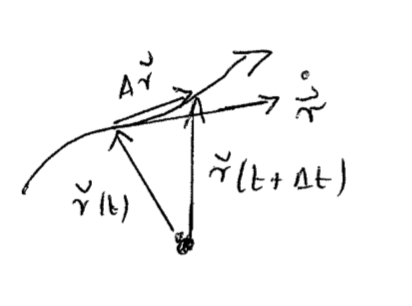
\includegraphics[scale=0.5]{Vektorfunktionen.png}
					\end{minipage}
					\hfill
					\begin{minipage}[t]{10cm}
						\vspace{0pt}
						$\vec{\dot{r}} = \frac{d\vec{r}}{dt}\\ = \lim_{\Delta t\to\ 0} \frac{\vec{r}(t + \Delta t) - \vec{r}(t)}{\Delta t} \\= (\frac{dx}{dt}, \frac{dy}{dt}, \frac{dz}{dt}) =$ Geschwindigkeit $\vec{v}$\\
						Beschleunigung = $\vec{a} = \frac{d\vec{v}}{dt} = \frac{d^2\vec{r}}{dt^2}$\\
					\end{minipage}
				\end{figure}
				\textbf{Kettenregel, Produktregel etc. gelten auf für Vektorfunktionen.}\\
				z.B.\\
				\[\frac{d}{dt}(\vec{a} \times \vec{b}) = \frac{d\vec{a}}{dt} \times \vec{b} \vec{a} \times \frac{d\vec{b}}{dt}\]
				\[ \frac{d}{dt}\vec{r} (f(t^\prime)) = \frac{d\vec{r}}{dt}(f(t^\prime)) * \frac{df}{dt^\prime}(t^\prime) \]
	\subsection{Integration}
	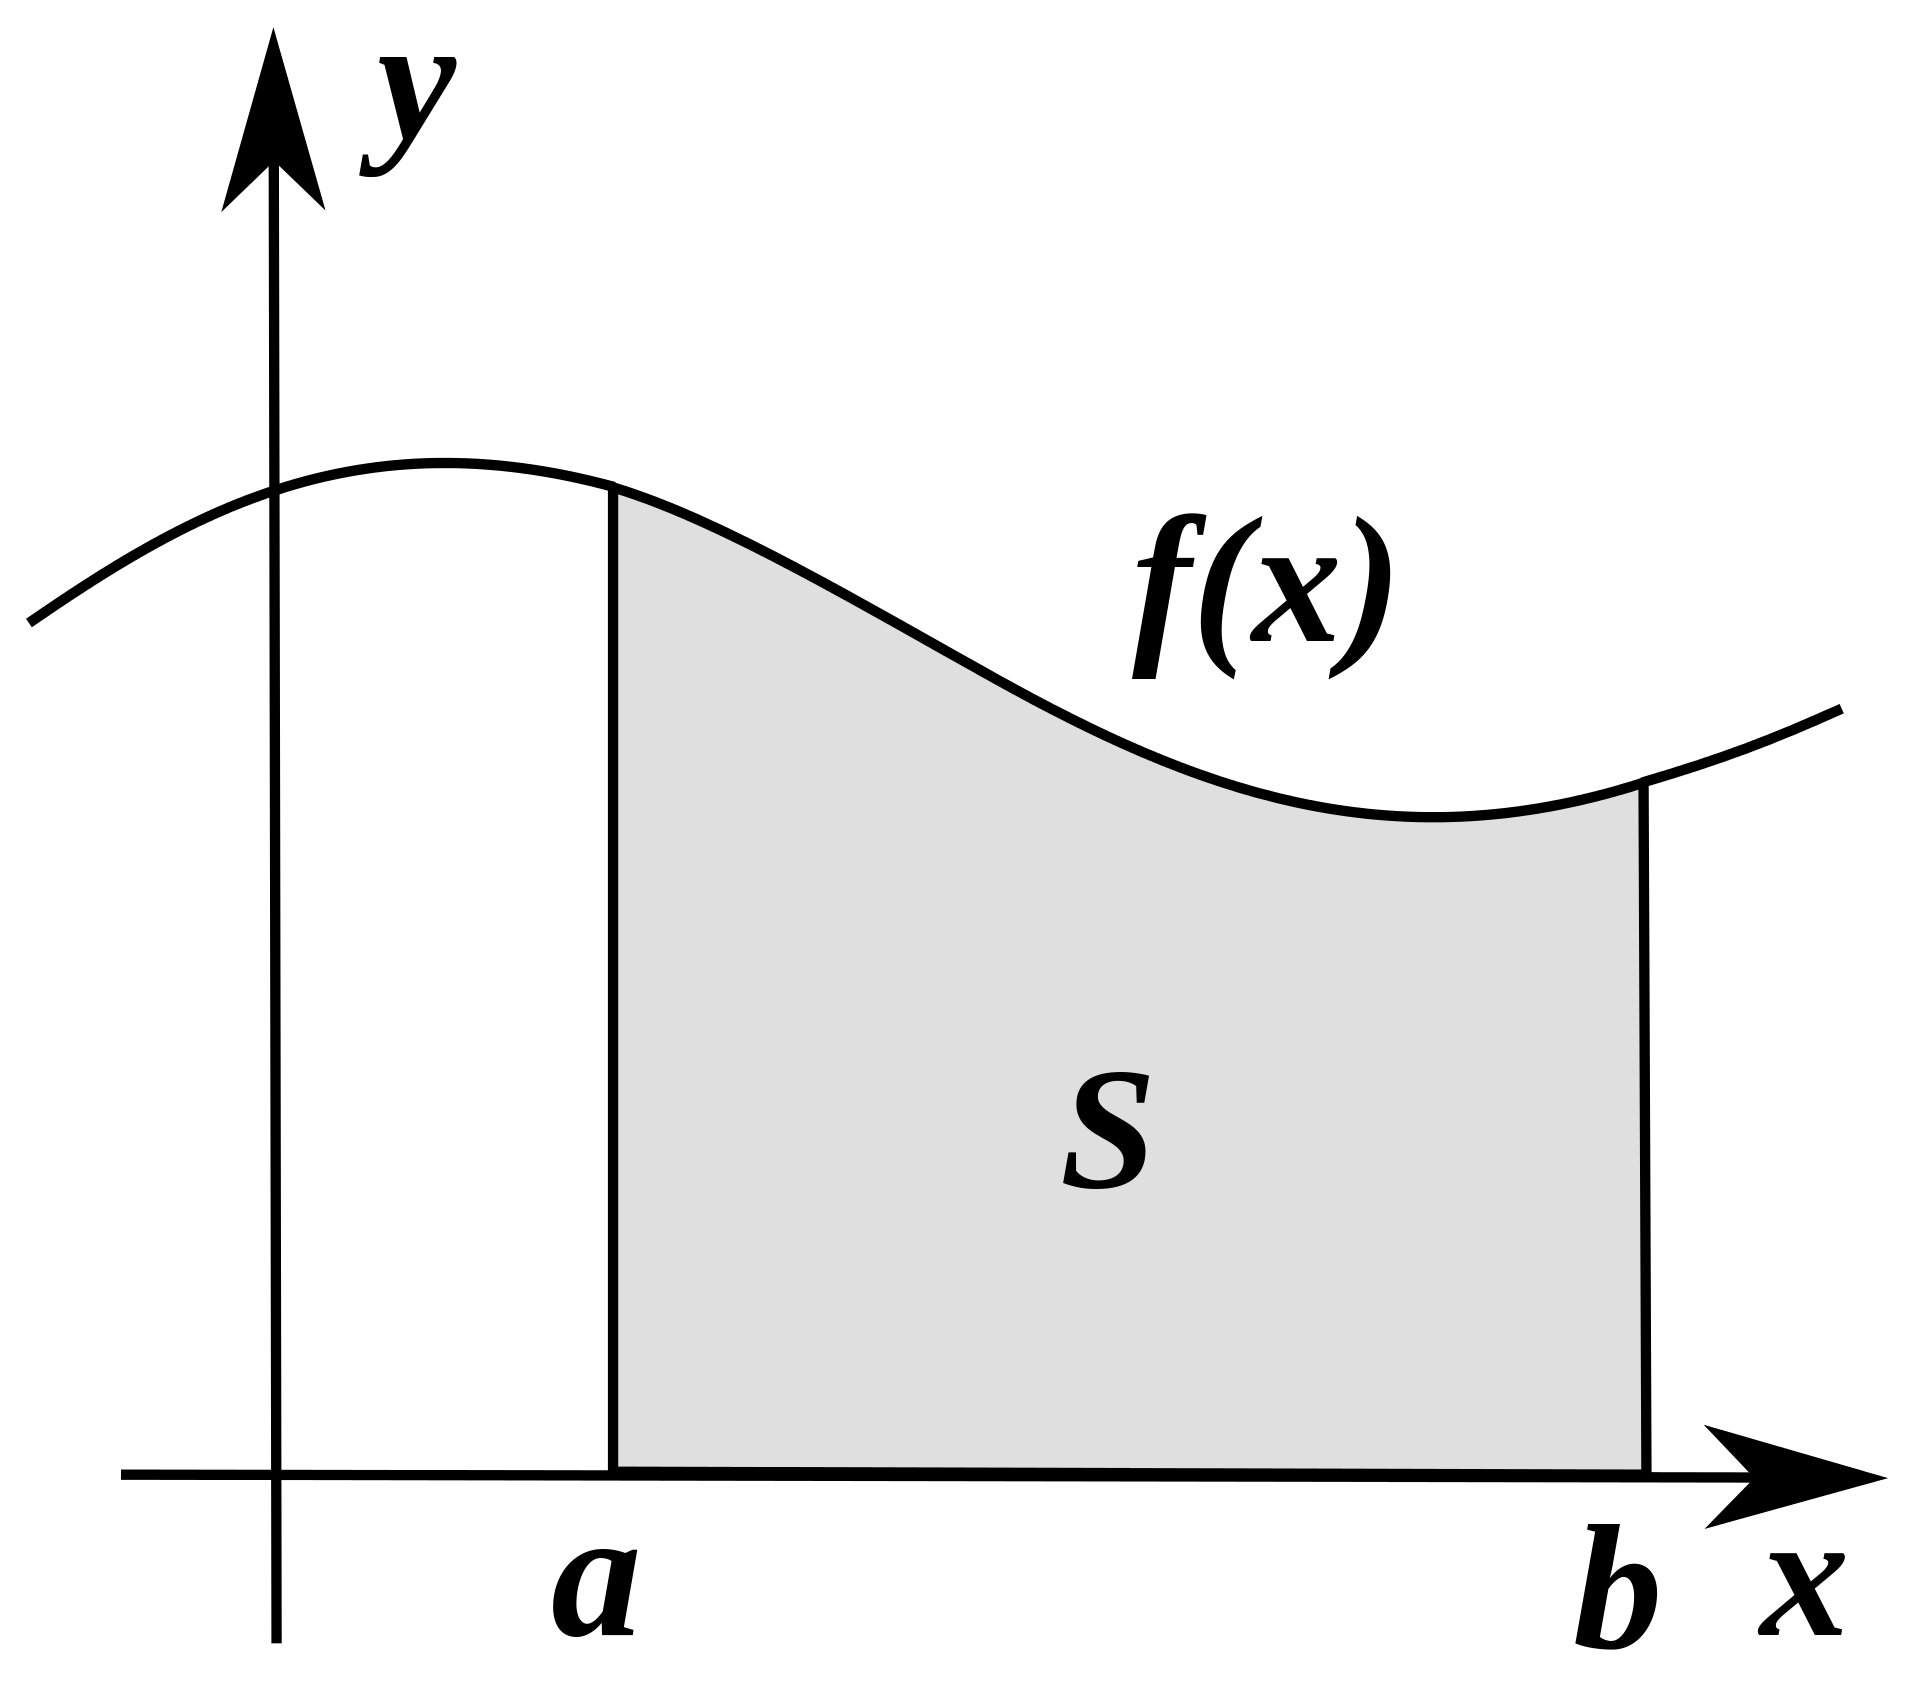
\includegraphics[scale=0.05]{integral.png}
	Die Integralrechnung ist aus dem Problem der Flächen- und Volumenberechnung entstanden.
	Dabei kann die Funktion auch ein komplett random geformter klotz in einem koordinaten System sein.\\
	$\int_a^b f(x)\,\mathrm dx$\\
	\begin{figure}[htbp]
		\begin{minipage}[t]{6cm}
			\vspace{0pt}
			\centering
			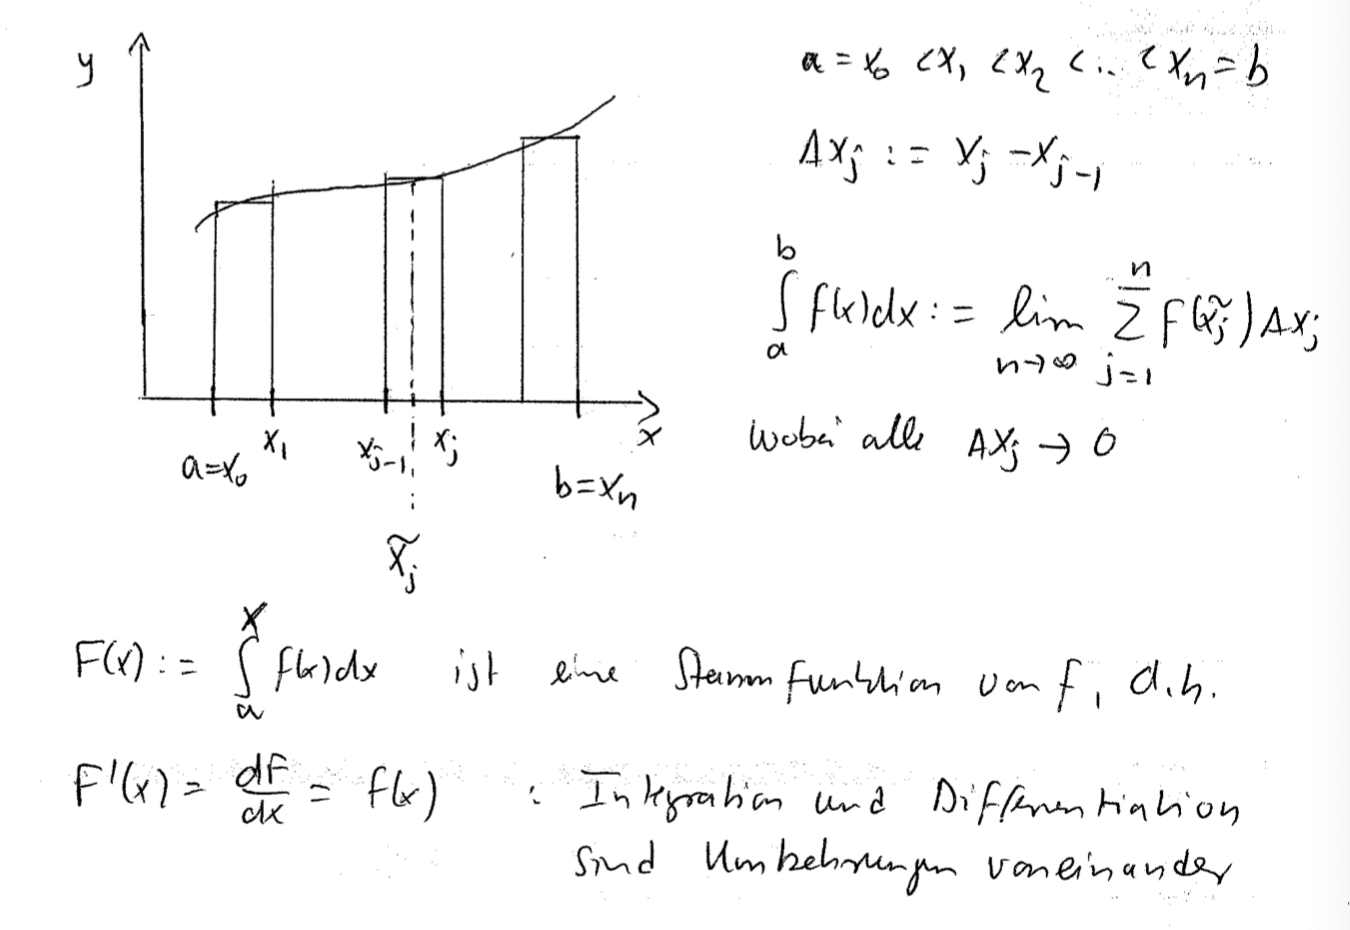
\includegraphics[scale=0.45]{Integrationbeispiel.png}
		\end{minipage}
		\hfill
		\begin{minipage}[t]{6cm}
			\vspace{0pt}
			Eine der am  häufigsten genutzen Regeln in der Physik ist, dass Konstanten vor das Integral gezogen werden können.
		\end{minipage}
	\end{figure}
\subsection{Differentialrechnung}
	\begin{center}
		$dy = df(x) = f^\prime(x)dx$
	\end{center}
	In der Mathematik wird dies Differentialform genannt, die man formal als dual zum Vektorraum bestehend aus Koordinaten $x, ...$ definiert.
	\newpage
	
	\part{Vorlesung 4}
	\subsection{Vektorfunktionen}
	z.B. Kurve eines Massenpunktes wird beschrieben durch $\vec{r}|t| = (x(t), y(t), z(t))$ wobei t die Zeit ist.\\
	\begin{figure}[htbp]
		\begin{minipage}[t]{10cm}
			\vspace{0pt}
			\centering
			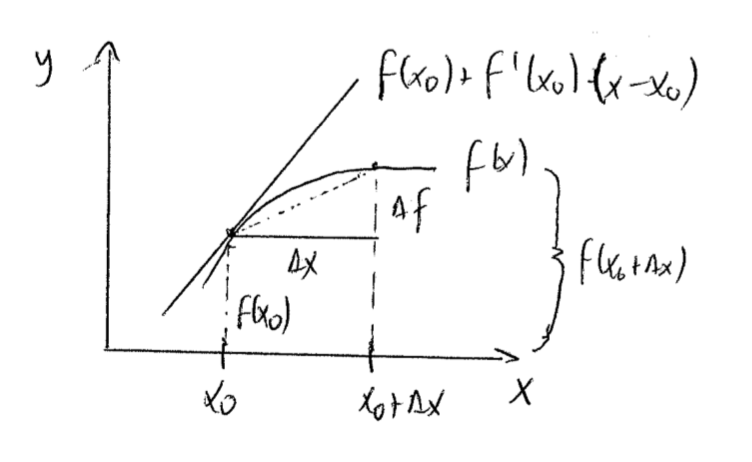
\includegraphics[scale=0.4]{Differentialrechnung.png}
		\end{minipage}
		\hfill
		\begin{minipage}[t]{10cm}
			\vspace{0pt}
			$f^\prime(x_0) = \frac{df}{dx} |_{x_0}$$ \\ = lim_{\Delta x \to\ 0} \frac{\Delta f}{\Delta x}\\ = lim_{x \to\ x_0} \frac{f(x) - f(x_0)}{x - x_0}$
		\end{minipage}
	\end{figure}
\subsection{Taylor Entwicklung}
	Im 1. Ordnung: $f(x) \approx f(x_0) + f^\prime(x_0)(x-x_0)$\\
\textbf{Verallgemeinerung}:\
	\[ f(x)= \sum_{n=0}^{\infty}\frac{f^(^n^) (x_0)}{n!} (x-x_0)^n = f(x_0) + f^\prime (x_0) (x - x_0) + \frac{f^\prime ^\prime (x_0)}{2} (x-x_0)^2 + ... \]
	\subsubsection{Potenzreihe}
	Jede \textbf{Potenzreihe} 
	$\sum_{n=0}^{\infty}a_n(x-x_0)^n$ und damit auch jede \textbf{Taylor-Reihe} hat einen Konvergenzradius $\lambda$, so daß $\sum_{n=0}^{\infty}a_n(x-x_0)^n$ für alle $|x-x_0| < r$ konvergiert. Im allgemeinen ist r durch den Abstand zur nöchsten Singularität von $f(x)$ gegeben, diese Tatsache gilt aber nur allgemein im Raum der komplexen Zahlen.\\
	\textbf{Beispiel}:\\ 
	$f(x) = \frac{1}{1 + x^2} = \sum_{n=0}^{\infty} (-1)^n x^2^n = \sum_{n=0}^{\infty} a_nx^n $ hat den Konvergenzradius $r = 1$, da $\frac{a_2_n_+_2}{a_2_n} = -x^2$ obwohl $\frac{1}{1+x^2}$ für alle $x \in \R$ wohldefiniert und unendlich oft differenzierbar ist. \\
	Der tiefere Grund ist daß $ \frac{1 }{1 + x^2} $ bei $x = \pm i$ singulär ist. 
	\subsection{Partielle Differentiation}
		Funktionen mehrerer Variablen, z.B. f(x,y,z), können nach den einzelnen Variablen differenziert werden, wobei man sich die anderen Variablen konstant vorstellt.\\
		\[ \frac{\partial f}{\partial x}(x,y,z) =  lim_{\Delta x \to\ 0} \frac{f(x+\Delta x,y,z - f(x,y,z))}{x,y,z} \]
		und analog für die anderen Variablen.\\ \textbf{Kurzschreibweise}:\\
		\[ f_x = \frac{\partial f}{\partial x} \quad f_y = \frac{\partial f}{\partial y} \quad f_z = \frac{\partial f}{\partial z} \] \\
		\subsubsection{Höhere Ableitungen}
		\[  f_x_x = \frac{\partial}{\partial x}(\frac{\partial f}{\partial x}) = \frac{\partial^2f}{\partial x^2} \]
	\[  f_x_y = \frac{\partial}{\partial y} (\frac{\partial f}{\partial x}) = \frac{\partial^2 f}{\partial_y \partial_x} \]
		 übrigens gilt: $\frac{\partial^2 f}{\partial y \partial x } = \frac{\partial^2 f}{\partial_x \partial_y}$ (Symmetrie)\\
		 Man kann leicht die erweiterte Kettenregel zeigen:\\
		 Für $f(t) = f(x|t) , y(t) , z(t)$ gilt $\frac{df}{dt} = \frac{\partial f}{\partial x} \frac{dx}{dt} frac{\partial f}{\partial y} \frac{dy}{dt} + frac{\partial f}{\partial z} \frac{dz}{dt}$\\ oder als Differential \\
		 $df = \frac{\partial f}{\partial x} dx + \frac{\partial f}{\partial y} dx + \frac{\partial f}{\partial z} dz   $\\
		 Kann auch für die 1. Ordnung einer multi-dimensionalen Taylor-Entwicklung verwendet werden: \\
		 $ f(x,y,z) = f(x_0, y_0, z_0) + \frac{\partial f}{\partial x} (x_0, y_0, t_0)(x-x_0) + \frac{\partial f}{\partial y} (x_0, y_0, t_0)(y-y_0) + \frac{\partial f}{\partial z} (x_0, y_0, t_0)(z-z_0) + ... $
	
		\subsection{Vektoranalysis: Gradient, Divergenz, Rotation}
			Ein \textbf{Vektorfeld} ist eine Vektor-wertige Funktion mehrerer Variablen:
			\[ \vec{F}(\vec{r}) = (F_x(x,y,z), F_y(x,y,z), F_z(x,y,z) ) \]
			\textbf{Beispiele:} Geschwindkeitsfeld (e.g. Windgeschwindigkeit), Kraftfeld\\
			Ein \textbf{Skalarfeld} hat nur eine (skalare) Komponente:
				\[ f(\vec{r}) = f(x,y,z) \]\\
				\subsubsection{Gradient}
				
				\[ f \rightarrow \vec{\nabla} f = grad f = \vec{\nabla} f = \left( \frac{\partial f}{\partial x}, \frac{\partial f}{\partial y}, \frac{\partial f}{\partial z} \right) \text{\qquad} Skalarfeld \rightarrow Vektorfeld \] 
				Es gelten die üblichen Produkt- und Summenregeln:
					\[ \vec{\nabla}(f+g) = \vec{\nabla }f + \vec{\nabla}g; \vec{\nabla}(f+g)= g\vec{\nabla}f + f\vec{\nabla}g \]
				\subsubsection{Beispiel}
				 f sei Funktion der Abstand $|\vec{r} - \vec{r}_0| = f^\prime (| \vec{r}-\vec{r}_0|) \frac{x-x_0}{| \vec{r} - \vec{r}_0 |}$ \\
				\textit{Dabei gilt:} $|\vec{r} - \vec{r}_0| = \sqrt{(x-x_0)^2 + (y-y_0)^2 + (z-z_0)^2}$\\
				Dabei ist das ganze dann logischer weise nur vom Abstand abhängig\\
				$\Rightarrow \vec{\nabla} (\vec{r}) =   \left( \frac{\partial f}{\partial x}, \frac{\partial f}{\partial y}, \frac{\partial f}{\partial z} \right) = \frac{1}{|\vec{r} - \vec{r}_0|} ( x-x_0, y- y_0, z- z_0 )    \frac{\vec{r} - \vec{r}_0}{| \vec{r}-\vec{r}_0 |} = \vec{e}_{\vec{r} - \vec{r}_0}$ \\
				\[ \frac{\partial r}{\partial x} = \frac{1}{2} \frac{2(x-x_0)}{\sqrt{(x-x_0)^2 + (y-y_0)^2 + (z-z_0)^2}} = \frac{x-x_o}{|\vec{r - \vec{r}_0}|} \]
				Einheiten in Kegelkoordinaten:\\
				$\Rightarrow \vec{\nabla} = \frac{df}{dr}(| \vec{r}-\vec{r}_0 |)  \vec{\nabla}| \vec{r}-\vec{r}_0 | = f^\partial (| \vec{r}-\vec{r}_0 |) \frac{\vec{r} - \vec{r}_0}{| \vec{r}-\vec{r}_0 |}$
				z.B. $ f(\vec{r}) = c | \vec{r}-\vec{r}_0 |  $ Das Gravitationspotential zwischen zwei Teilchen der Masse $m_1$ und $m_2$\\
				 $ \phi(\vec{r}_1 , \vec{r}_2) = -\frac{G_N m_1 m_2}{| \vec{r}-\vec{r}_0 |}$ $\alpha = -1$ und $c = -G_N m_1 m_2$\\
				 
				 $\Rightarrow  \vec{\nabla} \phi (| \vec{r}-\vec{r}_0 |) = \frac{G_N m_1 m_2}{| \vec{r}-\vec{r}_0 |} \frac{\vec{r} - \vec{r}_0}{| \vec{r}-\vec{r}_0 |} $ 
				 Nebenrechnung: $\phi^\partial (r) = + \frac{G_N m_1 m_2}{r^2}\\
				 \vec{F}_1_2 = - \vec{\nabla} \phi = - \frac{G_N m_1 m_2}{| \vec{r}-\vec{r}_0 |}(\vec{r} - \vec{r}_0)$ = Die Kraft die Teilchen 2 auf Teilchen 2 ausübt.
				
				\subsection{Rotation}
				Hierbei muss extrem auf die Vorzeichen aufgepasst werden. Es gibt zudem nur 2 Kombinationen wie man im laufe sehen wird die sich nicht wegkürzen.\\
					rot($\vec{F} (\vec{r}) = \vec{\nabla} \times \vec{F} = \sum_{i, j, k}^{}$ $\frac{\partial f_j}{\partial x_i}  \vec{e}_{i,j} = (\frac{\partial f_z}{\partial y} - \frac{\partial f_y}{\partial z}, \frac{\partial f_x}{\partial z} - \frac{\partial f_z}{\partial x}, \frac{\partial f_z}{\partial x} - \frac{\partial f_x}{\partial y}$)\\
					Es sind 3 da wir uns im 3 Dimensionalen befinden.  \quad  Vektorfeld $\Rightarrow$ Vektorfeld ; Wirbelstärke\\
					
					\subsubsection{Summe und Rotation}
						$\vec{\nabla} \times(\vec{F} + \vec{G}) = \vec{\nabla} \times \vec{F} + \vec{\nabla} \times \vec{G}$\\
						$ \vec{\nabla} \times(f \vec{F} )= f \vec{\nabla} \times \vec{F} (\vec{\nabla} f) \times \vec{F} $\\
					\subsubsection{Beispiel:}
							$f (\vec{r}) = \vec{F} = f(r) \vec{\nabla} \times \vec{r} + (\vec{\nabla} f) \times \vec{r}$\\
							$\vec{f} (\vec{r}) = (\frac{\partial f_z}{\partial y} - \frac{\partial f_y}{\partial z}, \frac{\partial f_x}{\partial z} - \frac{\partial f_z}{\partial x}, \frac{\partial f_z}{\partial x} - \frac{\partial f_x}{\partial y)} = \vec{0}  $ \qquad $\vec{r} = (x,y,z)$\\
							$\vec{\nabla}f = f^\prime \frac{\vec{r}}{|\vec{r}|} \Rightarrow (\vec{\nabla}f) \times \vec{r} = \frac{f^\prime}{|\vec{r}|} \times \vec{r} = 0$\\
							
							\subsubsection{Beispiel B}
							$\vec{F}(\vec{r}) = \vec{w} \times \vec{r}$\\
							$| \vec{F}(\vec{r})| = |\vec{w}| \sqrt{x^2+y^2}$\\
							$(\vec{\nabla}  \times \vec{F})_x = \frac{\partial f_z}{\partial y} - \frac{\partial f_y }{\partial z}  = \frac{\partial}{\partial y} (w_x y - w_y x) - \frac{\partial}{\partial z}(w_y x - w_x y)$ \\
							Damit gilt: $\vec{F} = \vec{w} \times \vec{a} \Rightarrow F_z = w_xy - w_yx$ und $F_y = w_zx - w_xz$\\
							Also ist es am ende: $\Rightarrow \vec{\nabla} \times \vec{F} = 2\vec{w}$\\
							
							
							$\Leftrightarrow \vec{\nabla} \times (\vec{w} \times \vec{r})= 2\vec{w}$
							
					\subsection{Divergenz}
						div $\vec{f} = \vec{\nabla}, \vec{F} = (\frac{\partial}{\partial x}, \frac{\partial }{\partial y} , \frac{\partial }{\partial z}) * F_x , F_y, F_z = \frac{\partial F_x}{\partial x} + \frac{\partial F_y}{\partial y}+ \frac{\partial F_z}{\partial z}$\\
						Vektorfunktion $\rightarrow$ Sklarafunktion\\
						$\vec{\nabla } (\vec{F} + \vec{G}) = \vec{\nabla} \vec{F} + \vec{\nabla} \vec{G} $ \quad $ \vec{\nabla}+ (f \vec{f}) = f \vec{\nabla} * \vec{F} +(\vec{\nabla f}) * \vec{F} $\\
						\subsubsection{Beispiele}
						$\vec{F} (\vec{r}) = \vec{r}$ \quad $\vec{\nabla} * \vec{r} = 3 $\\
						anderes Beispiel: $\vec{F} (\vec{r}) = \vec{w} \times \vec{r}$ \quad $\vec{w} = const.$\\
						wähle deine Einschränkungen: $\vec{w} = w\vec{e}_z = (0,0,w) \rightarrow \vec{w} \times \vec{r} = (-wy, wx, 0)$\\
						$\vec{\nabla} * (\vec{w} \times \vec{ r}) = \frac{\partial}{\partial x} (wx) + \frac{\partial}{\partial z} 0 = 0$\\
						Weitere Beispiele im im Skript.\\		
						\part{Vorlesung 5}				
					\subsection{Gradient und totales Differential}
						$f(x,y,z) \Rightarrow df = \frac{\partial f}{\partial x} dx +\frac{\partial f}{\partial y} dy+ \frac{\partial f}{\partial z} dz = (\vec{\nabla} f) * d\vec{ r}$\\
						$\vec{\nabla} f = \frac{\partial f}{\partial x}, \frac{\partial f}{\partial y} , \frac{\partial f}{\partial z}  \quad d\vec{ r} = (dx,dy,dz)$\\
						$\frac{df}{dt} = (\vec{\nabla} f) * \frac{d\vec{ r}}{dt} $\\
						$\Rightarrow$ $\int_{\vec{ r}_0}^{\vec{ r}_1} \frac{df}{dt} dt = \int_{\vec{ r}_0}^{\vec{ r}_1} (\vec{\nabla } f) d\vec{ r} = f(\vec{ r}_1) - f(\vec{ r}_0)$\\
						\subsubsection{Wegintegral eines Vektorfeldes $\vec{ F}(\vec{ r})$}
							Angenoimmen wir haben eine Kurve und wollen ein Kurvenintergral bilden und nennen dies dann c. Dabei ist der eine Endpun kt $\vec{ r}_0$ und $\vec{ r}_1$\\
							$\int_{c}^{} \vec{ F}(\vec{ r}) *d\vec{ r} = \int_{c}^{} [ F_x dx + F_y dy + F_z dz ] :=  \\ \lim_{N \to\ \infty}
							\sum_{i =1}^{N} \vec{ F}(\vec{ r}_i) * \Delta\vec{ r}_i = \lim_{N \to\ \infty} \sum_{i =1}^{N}\vec{ F}(\vec{ r}_i) * \frac{ \Delta \vec{ r}_i}{\Delta t} \Delta t$\\
							$\lim_{\Delta t\to\ 0} \Delta t_i = \lim_{N \to\ \infty} \Delta \vec{ r}_i = 0$\\
							Also zum Beispiel eine Arbeit, die durch einer Kraft $\vec{ F}(\vec{ r}) * d\vec{ r}$ verrichtet wird
								\[ W = \int \vec{ F}(\vec{ r}) * d\vec{ r} \]
								Dabei muss man sich immer den Kontext klar machen da sich dadurch ganz einfach Vorzeichen ändern können also der unterschied ob Arbeit verrichtet werden muss oder nicht. \textit{Zum Beispiel das Skalarprodukt würde sich daruch komplett ändern}\\
								\[ \int_{c_1} \vec{ F}(\vec{ r}) * d\vec{ r} \]
								\[ \int_{c_2} \vec{ F}(\vec{ r}) * d\vec{ r} \]
								diese Intergrale sind wegunabhängig $\Leftrightarrow \vec{ F} = \vec{\nabla } f \Leftrightarrow \vec{\nabla } \times \vec{ F} = 0$ \\
								\subsubsection{Eigenschaften:}
								$ \int_{-c} \vec{ F}* d\vec{ r} = -\int_{c} \vec{ F}*d\vec{ r}  $\\
								$ c = c_1 + c_2 \Rightarrow \int_{c}\vec{ F}*d\vec{ r} + \int_{c_2}\vec{ F}* d\vec{ r} $ 
					\subsection{Grundlagen der Dynamik}
						\textbf{Axiome der Newtonschen Mechanik}\\
						\begin{itemize}
							\item \textbf{1. Trägheitsgesetz:} Körper, auf den keine Kräte wirken, bewegt sich geleichförmig und gleichlinig, das heißt $ \vec{v} = const , \vec{v} = \vec{0}$ ist ein Spezialfall.
							\item \textbf{2. Aktionsprinzip} Die Zeitliche Änderung des Impulses $\vec{p}$ eines Körpers ist gleich der auf ihn einwirkenden Gesammtkraft
							\[ Impuls = m*\vec{v} = m\frac{d\vec{ r}}{dt} = \vec{p} \]
							\[ \vec{ F}_{total} = \frac{d\vec{p}}{dt} = \dot{\vec{p}} = m \dot{\vec{v}} = m \ddot{\vec{ r}} = m \vec{a} \]
							\item \textbf{3. Actio= Reactio} die von Körper 1 auf Körper 2 ausgeübte Kraft $\vec{ F}_{21}$ ist gleich dem negativen der von Körper 2 auf Körper 1 ausgeübte Kraft 
							\[ \vec{ F}_{21} = - \vec{ F}_{12} \]
							\item \textbf{Superpositionsprinzip} Kräfte addieren sich vektoriel.
						\end{itemize}
							In Newton´s Mechanik sind \textbf{Raum} und \textbf{Zeit} absolute Begriffe und die Zeit läuft immer gleich ab unabhängig vom Inertialsystem,  was natürlich in konflikt mit der Relativitätstheorie steht.\\
							Newtons Axiome gelten zunächst nur in unbeschleunigten, sog. Inertialsystemen. Intertialsysteme bewegen sich relativ zueinander mit konstanter Geschwindigkeit\\
							\subsubsection{Allgemeine Galilei- Transformation zwischen Inertialsystemen}
								\[ \vec{ r}^\prime = \vec{ r} + \vec{v}_0 * t + \vec{ r}_0 \qquad \vec{v}_0 = const ; \vec{ r}_0 = const \]
								Wie man sieht transformieren sich damit die Ortskoordinaten aber die Zeit bleibt offensichtlicherweise gleich.$t^\prime = t $ \
								\[ \vec{v}^\prime = \frac{d\vec{ r}^\prime}{dt} = \frac{d\vec{ r}}{dr} + \vec{v}_0 = \vec{v} + \vec{ v}_0 \]\
								\[ \vec{ a}^\prime = \frac{d^2\vec{ r}^\prime}{dt^2} = \frac{d^2\vec{ r}}{dt^2} = \vec{ a} \]
							\subsubsection{Galileisches Relativitätsprinzip}
								Newtonsche Bewegungsgleichung ist forinvariant unter Galileitransformation.
								\subsubsection{Exkurs Kosmologie}
									In der Kosmologie gibt es als \textit{bevorzugtes} Bezugssystem das Rugesystem der thermischen Mikrowellenhintergrundstrahlung.
									\subsubsection{Exkurs Machsches Prinzip}
										Existenz von Raum, Zeit und Intertialsystem ist beinflusst durch die Massenverteilung auf sehr großen (kosmologischen) Skalen.
									\subsubsection{Ausblick}
										\textbf{spezielle Relativitätstheorie:} Raum und Zeit werden relativ und die Galileitransofrmation werden durch Lorentztransformation ersetzt.\\
										\textbf{allgemeine Relativität}  Raum und Zeit (Geometrie) sind an die Materieverteilung gekoppelt. Das hat dann die Folge, dass die Teilchenbewegung bestimmt wird durchd ie Geometrie von Raum und Zeit. Die Massenverteilung bestimmt dann aber erst die Geometrie von Raum und Zeit.
							\subsubsection{Koordinatentransformationen - Krumlinige (räunliche) Koordinaten}
								Man habe n-Dimensionen $ (x_i) (y_i) \qquad |\leq i,y \leq n  $	
								\[ x_i = x_i(y_{y_1, ..., y_n}) = x_i(y_i) \]
								\[ dx_i = \sum_{j = 1}^{n} \frac{\partial x_i}{\partial y_y} dy_i \]
								\subsubsection{Beispiel}
									$ n=3$ mit $x_i =(x,y,z)$ Euklidische Kooridnaten; und $y_i = (u,v,w)$\\
									$x= x(u,v,w) \qquad dx = \frac{\partial x}{\partial u}du + \frac{\partial x}{\partial v} dv + \frac{\partial x}{\partial w} dw$\\
									$y = y(u,v,w) \qquad dy = \frac{\partial y}{\partial u}du + \frac{\partial y}{\partial v} dv + \frac{\partial y}{\partial w} dw$ und das gleiche für z.\\
									$\vec{r} = (x_1, ... , x_n) = (x_i) d\vec{ r}= (dx, ... , dx_n) = (dx_i) = \sum_{i} dx_i \vec{e}_i$ mit $ \vec{e}_i, \vec{e}_j = \delta_{i,j}$
							
							
							
							
							
							
							
\end{document}